\documentclass{beamer}
\usepackage[spanish]{babel}
\usepackage[utf8]{inputenc}
\usepackage{multicol}

\usepackage[
    type={CC},
    modifier={by-sa},
    version={3.0},
]{doclicense}


\usetheme{Warsaw}
\usecolortheme{crane}
\useoutertheme{shadow}
\useinnertheme{rectangles}

\setbeamertemplate{navigation symbols}{}

\title[XHTML y CSS]{Taller de XHTML y CSS3}
\subtitle{Nivel Básico - Parte II}
\author[Julián Fernández, Rubén Martín]{
	\textbf{Julian Fernández Ortiz }
	\\
	\medskip
	\scriptsize{
	Vicepresidente de IEEE Student Branch of Granada\\
	Grado en Ingeniería Electrónica Industrial
	}	
	\\	
	\texttt{julian.fernandez.es@ieee.org}
	\\ \ \\
	\small{\textbf{Rubén Martín Moreno}}
	\\
	\medskip
	\scriptsize{
	Tesorero de IEEE Student Branch of Granada\\
	Grado en Estadística
	}
	\\
	\texttt{ruben.martinmoreno.es@ieee.org}
}
\date{}

\begin{document}
\frame{\titlepage}

\begin{frame}
\frametitle{Licencia}
\doclicenseThis
Fuente: Curso desarrollado por IEEE Student Branch of Granada
\end{frame}

\begin{frame}
  \frametitle{Índice}
  \tableofcontents
\end{frame}

\section{CSS}
\begin{frame}[fragile]
\begin{columns}[t]
	\column{0.5\textwidth}
	Aplicar estilos localmente
	\column{0.5\textwidth}
	\scriptsize{
	\begin{verbatim}
	<body>
	  ...
	  <p style="color: red">TEXTO</p>
	  ...
	</body>
	\end{verbatim}
	}
	
\end{columns}
\end{frame}

\begin{frame}[fragile]
\begin{columns}[t]
	\column{0.5\textwidth}
	Establecer una hoja de estilos \textit{dentro del propio documento}
	\column{0.5\textwidth}
	\scriptsize{
	\begin{verbatim}
	<head>
	  ...
	  <style type ="text/css">
		h1{
			font-family: Algerian;
			color: #4113db; 
			font-style: italic ;
			text-align: center;
		  }
	  </style >
	  ...
	</head>
	\end{verbatim}
	}

\end{columns}
\end{frame}

\begin{frame}[fragile]
	Vincular una hoja de estilos externa\\ \ \\ (RECOMENDADO)
	\\ \ \\
	\scriptsize{
	\begin{verbatim}
	<head>
	  ...
	  <link href="style.css" rel="stylesheet" type="text/css" />
	  ...
	</head>
	\end{verbatim}
	}	
\end{frame}
	\subsection{Selectores}
\begin{frame}
	Una hoja de estilos es un archivo de texto que contiene reglas que determinan como se verán los elementos en la web. 
	\begin{itemize}
	\item Selector
	\item Declaración
	\end{itemize}
\end{frame}

\begin{frame}[fragile]
	\begin{columns}[c]
	\column{0.5\textwidth}
	\scriptsize{
	\begin{center}
	\begin{verbatim}
	selector{
	    propiedad1: valor1;
	    propiedad2: valor2;
	    ...
	}
	\end{verbatim}
\end{center}
	}
	\column{0.5\textwidth}
	\scriptsize{
	\begin{center}
	\begin{verbatim}
	h1{
	    color: gray;
	    font-family: "Corsiva Hebrew";
	}
	\end{verbatim}
	\end{center}
	}
\end{columns}
\end{frame}

\begin{frame}[fragile]
Es posible nombrar elementos para referirlos posteriormente:
	\begin{columns}[t]
	\column{5cm}
	\begin{block}{Elementos Únicos}
	\verb|       id="nombre"|
	\end{block}
	\column{5cm}
	\begin{block}{Grupo de Elementos}
	\verb|     class="nombre"|
	\end{block}
	\end{columns}
	\begin{itemize}
	\item Cada identificador deber ser único
	\item Más de un elemento puede pertenecer a la misma clase
	\end{itemize}
\end{frame}

\begin{frame}[fragile]
Hay varias formas de definir selectores
\begin{columns}[t]
	\column{0.5\textwidth}
	\begin{itemize}
	\item \verb|h1 {color: red;}|
	\item \verb|em.class {color: red;}|
	\item \verb|em#id {color: red;}|
	\item \verb|h1 em {color: red;}|
	\item \verb|a:link {color: red;}|
	\end{itemize}
	\column{0.5\textwidth}
	\begin{itemize}
	\item Normal
	\item Con clase
	\item Con identificador
	\item Jerárquicos
	\item Basado en estado
	\end{itemize}
\end{columns}
\end{frame}

\begin{frame}[fragile]
Para cambiar el estilo de varios selectores a la vez usamos comas:
	\begin{center}
	\begin{verbatim}
	h1,h2,h3{
	    color: red;
	}
	\end{verbatim}
	\end{center}
Para cambiar el estilo de todos los selectores usamos *:
	\begin{center}
	\begin{verbatim}
	*{
	    color: red;
	}
	\end{verbatim}
	\end{center}
\end{frame}
	\subsection{Diseño}
\begin{frame} %Elementos
Para estructurar la página debemos dividirla en secciones lógicas
	\begin{itemize}
	\item Elementos div
	\item Elementos span
	\end{itemize}
\end{frame}

\begin{frame} %Elementos
\frametitle{Estructura}
La estructura comúnmente utilizada es:
	\begin{itemize}
	\item \textbf{conteiner} o contenedor
	\item \textbf{header} o cabecera
	\item \textbf{content} o contenido
	\item \textbf{footer} o pie
	\end{itemize}
	\begin{exampleblock}{CONSEJO}
	Esta estructura es la más común, pero puedes usar la que te resulte más sencilla
	\end{exampleblock}
\end{frame}

\begin{frame} %Modelo de cajas
\frametitle{Modelo de Cajas}
	\begin{center}
	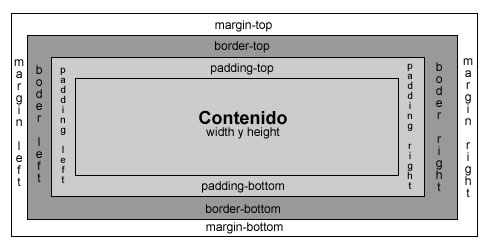
\includegraphics[scale=.5]{images/ModeloCajas.jpg} 
	\end{center}
\end{frame}

\begin{frame} %Modelo de cajas - Posición
\frametitle{Modelo de Cajas}
	Posicionamiento de una caja:
	\begin{itemize}
	\item Estático
	\item Absoluto
	\item Fijo
	\item Relativo
	\end{itemize}
\end{frame}

\begin{frame} %Propiedad FLOAT
\frametitle{Elementos Flotantes}
	Un elemento puede ``flotar'' a la derecha o a la izquierda usando la propiedad {\tt float}.
	\begin{center}
	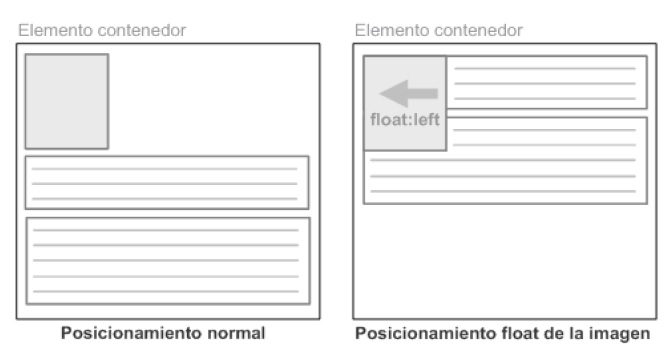
\includegraphics[scale=.5]{images/Floats.jpg} 
	\end{center}
\end{frame}

\begin{frame} %Estructura de cajas
	\begin{columns}[c]
	\column{0.7\textwidth}
	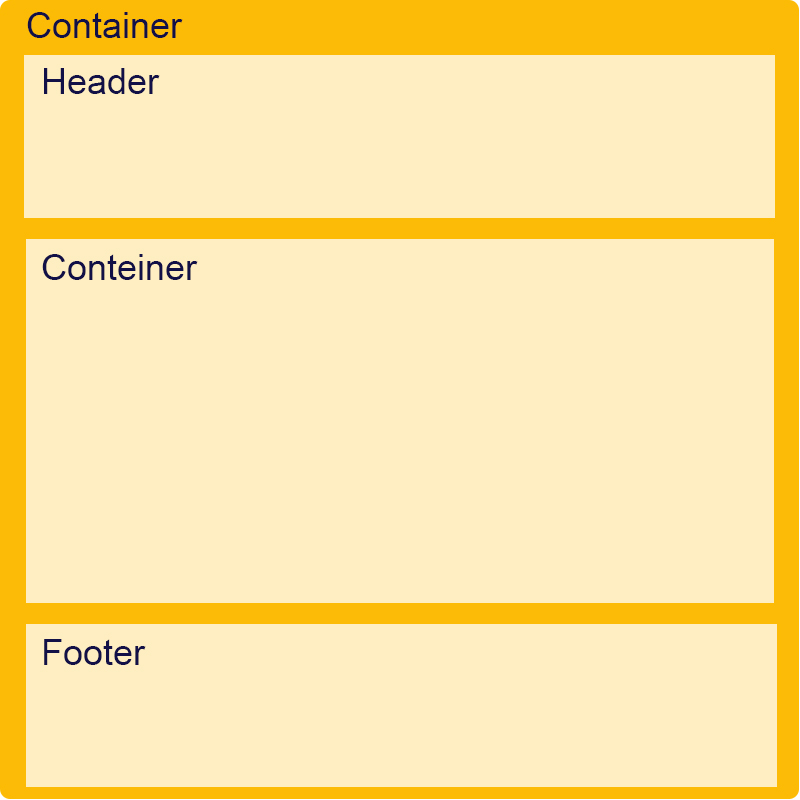
\includegraphics[scale=.22]{images/PruebaEstructura.jpg} 
	\column{0.3\textwidth}
	Estas estructuras se dividen con {\tt <div>...</div>}
	\end{columns}
\end{frame}


	\subsection{Colores y Fondo}
\begin{frame}
Sistemas más comunes
	\begin{columns}[c]
	\column{0.5\textwidth}
	\begin{itemize}
	\item RGB(a)
	\item Hexadecimal
	\end{itemize}
	\column{0.5\textwidth}
	\begin{exampleblock}{RECUERDA}
	También puedes definir el color usando su nombre
	\end{exampleblock}
	\end{columns}
\end{frame}

\begin{frame} % RGB - HEX
\definecolor{col1}{RGB}{0,0,0}
\definecolor{col2}{RGB}{255,0,0}
\definecolor{col3}{RGB}{0,255,0}
\definecolor{col4}{RGB}{0,0,255}
\definecolor{col5}{RGB}{255,255,0}
\definecolor{col6}{RGB}{0,255,255}
\definecolor{col7}{RGB}{255,0,255}
\definecolor{col8}{RGB}{192,192,192}

\begin{center}
\begin{tabular}{cc}
\frametitle{Colores RGB y HEX}
\textbf{RGB} & \textbf{HEX} \\
\colorbox{col1}{\makebox (120,12){\textcolor{white}{0,0,0}}} & \colorbox{col1}{\makebox (120,12){\textcolor{white}{\#000000}}} \\ 
\colorbox{col2}{\makebox (120,12){255,0,0}} & \colorbox{col2}{\makebox (120,12){\#FF0000}} \\
\colorbox{col3}{\makebox (120,12){0,255,0}} & \colorbox{col3}{\makebox (120,12){\#00FF00}} \\ 
\colorbox{col4}{\makebox (120,12){0,0,255}} & \colorbox{col4}{\makebox (120,12){\#0000FF}} \\ 
\colorbox{col5}{\makebox (120,12){255,255,0}} & \colorbox{col5}{\makebox (120,12){\#FFFF00}} \\ 
\colorbox{col6}{\makebox (120,12){0,255,255}} & \colorbox{col6}{\makebox (120,12){\#00FFFF}} \\ 
\colorbox{col7}{\makebox (120,12){255,0,255}} & \colorbox{col7}{\makebox (120,12){\#FF00FF}} \\ 
\colorbox{col8}{\makebox (120,12){192,192,192}} & \colorbox{col8}{\makebox (120,12){\#C0C0C0}} \\ 
\end{tabular} 
\end{center}
\end{frame}

\begin{frame}[fragile] %Fondo
\frametitle{Fondo}
	Propiedades comunes que se utilizan para personalizar el fondo de la página:
	\begin{itemize}
	\item \verb|background-attachement|
	\item \verb|background-color|	
	\item \verb|background-image|
	\item \verb|background-position|
	\item \verb|background-repeat|
	\end{itemize}
\end{frame}

	\subsection{Texto}
\begin{frame}[fragile]
	Atributos comunes que se utilizan para personalizar el texto:
	\begin{multicols}{2}
	\begin{itemize}
	\item \verb|font-family|
	\item \verb|font-style|
	\item \verb|font-variant|
	\item \verb|font-weight|
	\item \verb|font-size|
	\item \verb|text-align|
	\item \verb|text-decoration|
	\item \verb|text-indent|
	\item \verb|text-justify|
	\item \verb|text-overflow|
	\item \verb|text-transformation|
	\end{itemize}
	\end{multicols}
\end{frame}

	\subsection{Enlaces}
\begin{frame}[fragile] %Enlaces - EDICIÓN
\frametitle{Tipos de Enlaces}
	Existen 4 atributos que se utilizan para editar los enlaces:
	\begin{itemize}
	\item \verb|:link|
	\item \verb|:visited|
	\item \verb|:hover|
	\item \verb|:active|
	\item \verb|:focus|
	\end{itemize}
	Además se pueden completar con más atributos, como por ejemplo \verb|target|
\end{frame}

	\subsection{Listas, Cajas y Tablas}
\begin{frame}[fragile] %Listas
\frametitle{Listas}
	A la hora de editar una lista tendremos en cuenta de si esta es \textit{ordenada} o \textit{desordenada}
	\begin{itemize}
	\item \verb|list-style-type|
	\item \verb|list-style-position|
	\item \verb|list-style-image|
	\end{itemize}
\end{frame}

\begin{frame}[fragile] %Cajas
\frametitle{Cajas - Bordes}
	\begin{columns}[c]
	\column{0.55\textwidth}
	Algunos atributos utilizados
	\begin{itemize}
	\item \verb|border-color|
	\item \verb|border-style|
	\item \verb|border-width|
	\item \verb|border-radius|
	\end{itemize}
	
	\begin{exampleblock}{RECUERDA}
	Puedes editar solo un lado del borde haciendo referencia con el código \verb|border-top|, \verb|border-right|, \verb|border-bottom| o  \verb|border-	left|
	\end{exampleblock}
	\column{0.45\textwidth}
	\begin{center}
	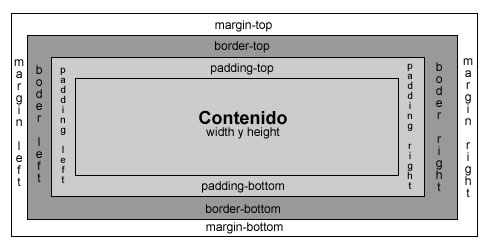
\includegraphics[scale=.3]{images/ModeloCajas.jpg} 
	\end{center}
	\end{columns}
\end{frame}

\begin{frame}[fragile] %Tablas
\frametitle{Tablas}
	Para editar los bordes de las celdas ya sean pertenecientes a toda la tabla, los encabezados o al cuerpo de la tabla
	\begin{itemize}
	\item \verb|border-collapse|
	\item \verb|border-spacing|
	\item \verb|caption-side|
	\item \verb|empty-cells|
	\end{itemize}
\end{frame}
	\subsection{Efectos Dinámicos}
\begin{frame}[fragile] %Preámbulo
	Los estilos CSS nos ayudan a crear efectos dinámicos sin la utilización de \verb|scripts|
	
	Algunos ejemplos son:
	\begin{itemize}
	\item Botones
	\item Menús desplegables
	\item Pop-ups
	\item ...
	\end{itemize}
\end{frame}
	
\section{BIBLIOGRAFÍA}
\begin{frame}
	http://www.w3c.es/estandares/
	
	http://www.w3schools.com/
	
	http://www.javascripter.net/faq/rgbtohex.htm
	
	http://librosweb.es/
\end{frame}

\end{document}
